In this chapter we will introduce the notations and concepts we will use in subsequent sections.

\todo{Introductions to used classifiers, concepts}
\todo{Concretize the problem and its notation}

\labelsubsection{Classification Task}{subsec:classification_task}
Classification in machine learning is the task of automatically assigning classes, or labels, to datapoints.
Given a dataset $D = \{(x_1, y_1), (x_2, y_2), \ldots, (x_n, y_n) \} \subseteq X \times Y$ of $n$ items where $(x_i, y_i)$ are dataset instances, the supervised classification task is to create a classifier which predicts a label $y' \in Y$ for a given $x \in X$.
In this work, the labels $Y$ of the dataset are denoted with $Y_d = (y_1, y_2, \ldots, y_n )$, the predicted labels are denoted as $Y'_d = (y'_1, y'_2, \ldots, y'_n )$.
When the number of classes $|Y|$ is 2, the classification task is also called binary classification. When $|Y$ is greater than 2, the classification is called multiclass classification.
In our case, the datapoints $x_i$ will be texts or graphs, therefore our task is called text and graph classification respectively.

\begin{figure}[ht]
\centering
\begin{tabular}{lll}
 & Notation & Definition \\
\toprule
Datapoint & $x$ & $x \in X$
\\
Label & $y$ & $y \in Y$
\\
Real and predicted label of $x_i$ & $y_i$, $y'_i$ &  $y_i, y'_i \in Y$
\\
Instance & $d_i$ & $(x_i, y_i) \in X \times Y$
\\
Dataset & $D$ & $\{(x_1, y_1), \ldots, (x_n, y_n) \} \subseteq X \times Y$ 
\end{tabular}
\caption{Classification notation.}
\end{figure}

The performance of a classifier is evaluated by comparing the predicted labels $y'_i$ for all datapoints $x_i$ with the real label $y_i$ in the dataset.
There are several metrics for evaluating the performance of a classifier.
The metrics we use in this work are summarized in Figure \ref{fig:classification_metrics}.

\begin{figure}[ht]
\centering
\renewcommand*{\arraystretch}{2.1}
\begin{tabular}{llll}
 & Notation & Definition & \\
\toprule
True positives of $y$ &
$TP_y$ &
$\displaystyle |\{i | y'_i = y, y'_i = y_i \}|$ &
\\
False positives of $y$ &
$FP_y$ &
$\displaystyle |\{i | y'_i = y, y_i \neq y \}|$ &
\\
True negatives of $y$ &
$TN_y$ &
$\displaystyle |\{i | y'_i \neq y, y_i \neq y\}|$ &
\\
False negatives of $y$ &
$FN_y$ &
$\displaystyle |\{i | y'_i \neq y, y_i = y\}|$ &
\\
\midrule
Accuracy &
$A$ &
$\displaystyle \frac{\sum\nolimits_{y \in Y} TP_y}{|D|}$ &
\\
Precision of $y$ &
$Pr_y$ &
$\displaystyle \frac{TP_y}{TP_y + FP_y} $ &
$Pr_{\text{macro}} = \displaystyle \frac{\sum\nolimits_{y \in Y} Pr_y}{|Y|}$
\\
Recall of $y$ &
$R_y$ &
$\displaystyle \frac{TP_y}{TP_y + FN_y}$ &
$R_{\text{macro}} = \displaystyle \frac{\sum\nolimits_{y \in Y} R_y}{|Y|}$
\\
F1 score of $y$ &
$F1_y$ &
$\displaystyle 2 \cdot \frac{Pr_y \cdot R_y}{Pr_y + R_y}$ &
$F1_{\text{macro}} = \displaystyle \frac{\sum\nolimits_{y \in Y} F1_y}{|Y|}$
\\
\end{tabular}
\caption{Classification performance metric notation. As performance metrics, we will us accuracy, macro precision, macro recall and the macro F1 score. The macro version of a metric takes into account how many elements there are in each class which is helpful for skewed datasets, ie. where the number of instances per label is not distributed uniformly per label.}\label{fig:classification_metrics}
\end{figure}


\labelsubsection{Texts}{subsec:texts}
\todo{Mention approaches to represent text}

\labelsubsection{Graphs}{subsec:graphs}
A labeled graph is a triple $G = (V, E, \pi)$, where $V$ is the set of vertices or nodes, $E \subseteq V \times V$ are the edges and $\pi: V \to X$ is a labeling function which assigns a label to a given vertex.

A graph is called undirected when $\forall (v_1, v_2) \in E: (v_2, v_1) \in E$, otherwise it is called directed.

A graph $G'=(V', E', \pi)$ is called a subgraph of graph $G = (V, E, \pi)$ when $V' \subseteq V$, $E' \subseteq E$ and $\forall (v, v') \in V': v \in V' \land v' \in V'$.

The (outgoing) neighbours $n(v)$ of a node $v$ are defined as the set $n(v) = \{v' | (v, v') \in E \}$.

\paragraph{Walks and Paths}
A walk on a graph is a (finite) sequence of edges, $w = (e_1, \cdots, e_n)$ with the constraint that $\forall 0 < i < n: \forall e_i = (v_1, v_2) \in w: \exists v_3: e_{i + 1} = (v_2, v_3)$. The length of the walk is $n$.
The set of all possible walks is denoted $W_G$.
A random walk starting from vertex $v$ is a walk where the first element of walk $w$ is $e = (v, v')$ for some $v'$.

A path is the sequence of the vertices visited on a walk, ie. for the walk $w = ((v_1, v_2), (v_2, v_3), \dots, (v_{n-1}, v_n)$, the path is $(v_1, v_2, v_3, \dots, v_n)$.
The set of all possible paths is denoted $P_G$.

The distance $d_{istance}(v, v')$ between two vertices is defined as the length of the shortest path between them.

\paragraph{Connected components}
A connected component $c$ of a graph is a set of vertices with the constraint $\forall v, v' \in c: \exists p \in P_G: v \in p \land v' \in p$, ie. there exists a path between every vertex in the connected component.
The connected component $c_v$ of a vertex $v$ is the connected component $c$ of a graph where $v \in c$.
The set of all connected components of a graph is $c_{all}(G) = \{ c_v | v \in V \}$. A graph is called connected when there is only one connected component. Only the empty graph has zero connected components.

\paragraph{Degree}
The in-degree $d_{in}$ of a vertex $v \in V$ is $d_{in}(v) = |\{v | (v_1, v_2) \in E \land v_2 = v\}|$.
The out-degree $d_{out}$ is defined analogously as $d_{out}(v) = |\{v | (v_1, v_2) \in E \land v_1 = v\}|$.
The degree of a vertex $v$ is $d(v) = d_{in}(v) + d_{out}(v)$ for directed graphs, and $d(v) = degree_{in}$ for undirected graphs.

\begin{figure}[ht]
\centering
\begin{tabular}{ll}
symbol &  meaning \\
\midrule
G & Graph \\
$E$ & Set of edges \\
$V$ & Set of vertices \\
$\pi(v)$ & Vertex labeling function \\
$n(v)$ & Neighbours of vertex $v$ \\
$W$ & All possible graph walks on graph $G$ \\
$w$ & Graph walk \\
$P$ & All possible paths on graph $G$ \\
$p$ & Path \\
$d(v)$ & Degree of vertex $v$ \\
$d_{in}(v)$ & In-degree of vertex $v$ \\
$d_{out}(v)$ & Out-degree of vertex $v$ \\
$d_{istance}(v, v')$ & Shortest path length between $v$ and $v'$ \\
$c_{all}(G)$ & Set of all connected components of $G$ \\
$c(v)$ & Connected component of $v$ \\
\end{tabular}
\caption{Graph notation.}
\end{figure}

\subsubsection{Concept Map}
A concept map is a (directed) graph where the nodes are concepts.
Concepts are important tokens in the text and consist of one or more words of the underlying text.
An edge between two concepts show that these concepts are related to each other. Edges can have labels also.
For an example of a concept map, see Figure \ref{fig:concept_map}.

\begin{figure}[ht]
\centering
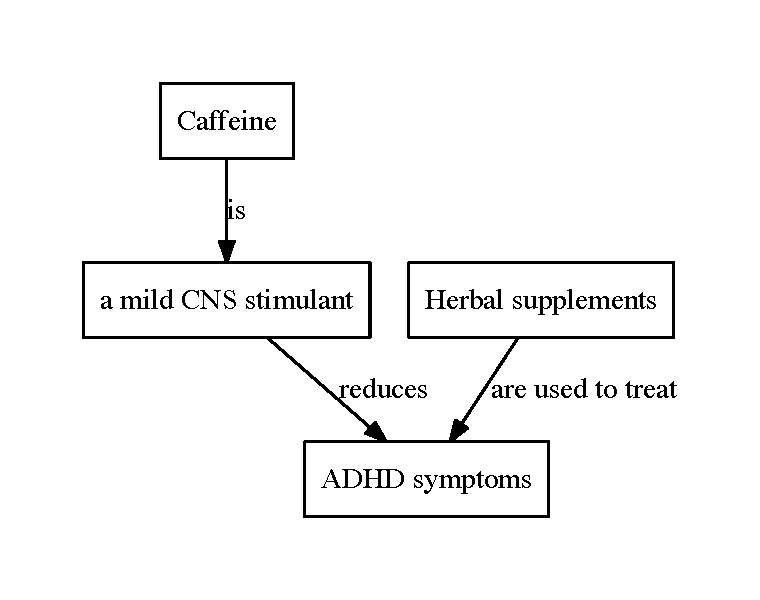
\includegraphics[width=0.5\linewidth]{assets/figures/concept_map.pdf}
\caption{Example of a concept map. The nodes are the concepts. The directed edges connect the concepts to each other and have labels. In this example of a concept map, one could recover sentences from this graph, for example ``Caffeine \textit{is} a mild CNS stimulant". Taken and adapted from: \cite{Falke2017}}
\label{fig:concept_map}
\end{figure}

Concept maps are useful for visualizing concepts and their relation to each other.
Concept maps can be used to quickly explore a given topic and immediately see connections between concepts.
Through the degree of a concept, one can also infer the relative importance of that concept in the underlying text.

By combining different texts of the same topic, one can also create a concept map for the whole topic.
In this case, the concepts are not confined to a single text.

The visualization with concept maps of one or more individual texts therefor enables the non-linear exploration of multiple texts of a topic at the same time.

Since the concepts in a concept map often contain only a small subset of the text, concept maps also summarize the underlying text.
Only relevant concepts and their relation to each other are captured, making concept maps interesting for (multi-document) text summarization.

In Chapter \ref{sec:implementation} we introduce the concept map extraction implementation we used and further explain the steps in creating the concept maps.

\subsubsection{Co-Occurrence Graph}
A co-occurrence graph, or graph-of-words, is generated from a text by creating a (directed) graph with all the words of the underlying text as nodes.
There is an edge between two nodes if the labels of the source and target node co-occur in the text.
Two words co-occur when the distance between the words in the text is below a given threshold, the window size.
Co-occurrence graphs can have edge weights corresponding to the counts of the co-occurrence of the words in the text.

Figure \ref{fig:cooccurrence_graphs} shows examples of co-occurrence graphs with different windows sizes.

\begin{figure}[ht]%
    \centering
    \subfloat[Window size: 1]{{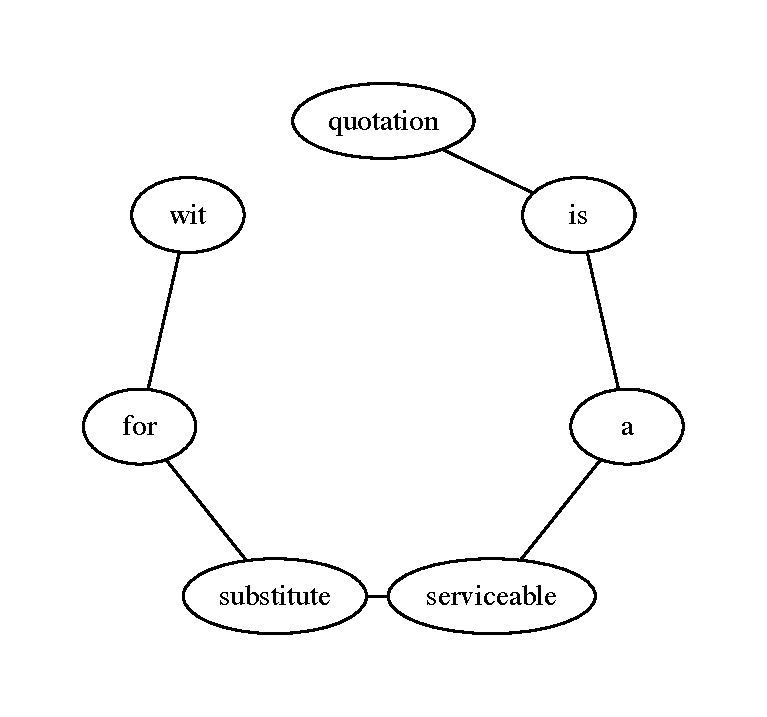
\includegraphics[width=0.3\textwidth]{assets/figures/cooccurrence/window_size_1.pdf} }}%
    \subfloat[Window size: 2]{{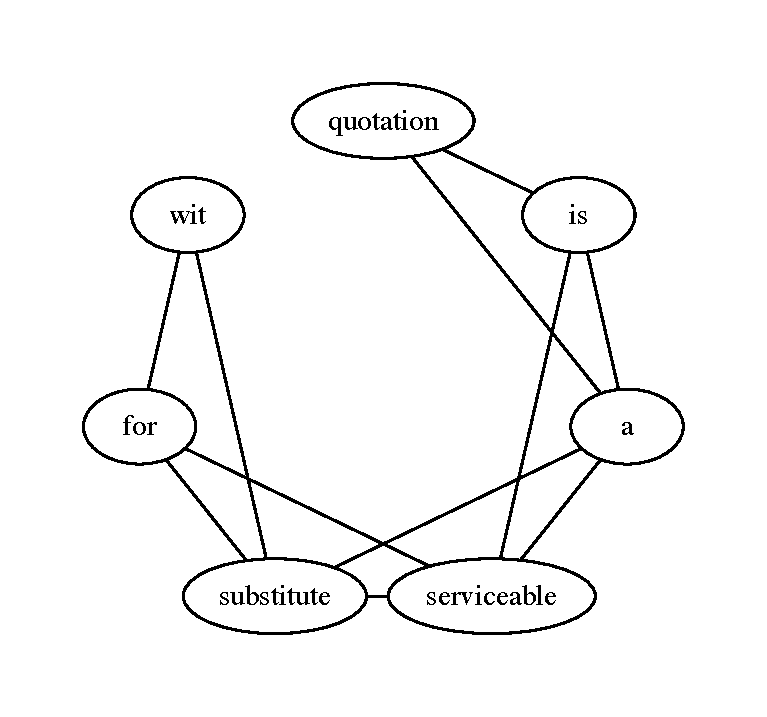
\includegraphics[width=0.3\textwidth]{assets/figures/cooccurrence/window_size_2.pdf} }}%
    \subfloat[Window size: 6]{{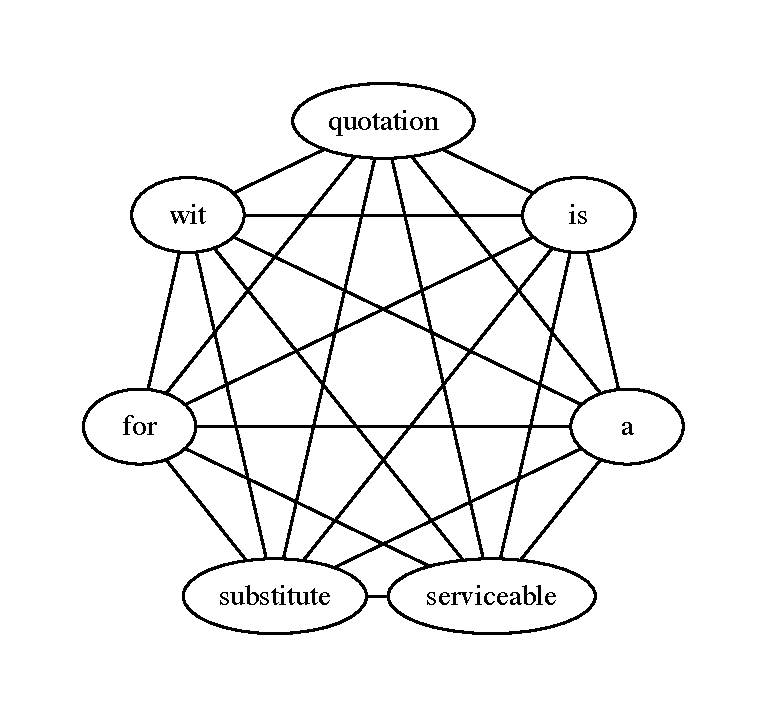
\includegraphics[width=0.3\textwidth]{assets/figures/cooccurrence/window_size_6.pdf} }}%
    \caption{Example for co-occurrence graphs. Generated from the sentence: ``Quotation is a serviceable substitute for wit". With increasing window size, the number of edges and therefor the connectedness of the co-occurrence graph also increases.}%
    \label{fig:cooccurrence_graphs}%
\end{figure}

Since co-occurrence graphs not only contain the words of the underlying text but also their co-occurrence, they capture not only the content of the text but also the relation between words of the text.
Therefor they contain structural information about the text.
Because of their similarity to concept maps, we will use co-occurrence maps as a baseline for the graph classification.
It has to be noted that this comparison is not entirely fair since co-occurrence graphs contain all words of the text and there is only a small loss of information.
The concept maps we extracted on the other hand have a far greater compression factor as we will see, ie. they summarize the content more.
For our comparison, we will also not use the edge weights since concept maps do not have edge weights.

\labelsubsection{Graph Kernel}{subsec:graph_kernel}
In most cases, texts and graphs are not of fixed size.
However, most classification algorithms operate on fixed size vectors.
Fortunately, there are several approaches to overcome this problem.
One of the approaches to nevertheless classify non-fixed size objects are so-called kernels.

A kernel is a function $k$ which returns a measure of similarity between two objects:
\begin{equation*}
k: X \times X \rightarrow \mathbb{Q}
\end{equation*}

A kernel function has to be:
\begin{itemize}
    \item{\textit{symmetric}: $k(x, x') = k(x', x)$}
    \item{\textit{non-negative definite}: $\forall x, x': k(x, x') \geq 0$}
\end{itemize}

An interesting property of kernels is that they can be combined easily with symmetric operations, eg. by adding or multiplicating the results of two kernel functions, $k_1$ and $k_2$:

\begin{equation*}
k_{combined}(x, x') = k_1(x, x') \cdot k_2(x, x')
\end{equation*}

One can easily confirm that when $k_1$ and $k_2$ are valid kernels, $k_{combined}$ is also a valid kernel.
This property enables composite kernels to capture multiple means of similarity in one metric.

For example, a simple kernel on two numbers (or vectors) is $k(x, x') = | x \cdot x' |$, where $| \cdot |$ is the absolute value (or a norm).
Another example of a kernel between strings is $k(s, s') = \delta(s = s')$, where $\delta(\cdot)$ is the Kronecker delta. This kernel returns 1 if the two given strings are the same, and 0 if they are different.
Note that both these kernels are indeed valid.

Kernel functions can be used in kernel methods for classification and other tasks.
Prominent examples of kernel methods are the SVM, kernelized PCA and Gaussian Processes.

For a subset of kernels, one can also create explicit feature vectors for a given object. In this case, the kernel can be written as an inner product on two fixed-size vectors:

\begin{equation*}
    k(X, X') = \langle \phi(X), \phi(X') \rangle
\end{equation*}

Here, $\phi(X)$ returns a fixed-size vector representation of the object $X$ and is the main part of the kernel.
This $\phi(X)$ can then be used in all vector-based classification algorithms, not only kernel methods.
An example for such a kernel is the string kernel which counts the number of occurrences of words in a given text, then creates a vector representation by giving each word an index in the vector and setting this index to the number of occurrences of that word. The inner product of two of these vector representations then create a kernel.

A graph kernel is simply a kernel that operates on graphs.

Graph kernels that measure the similarity of two graphs are related to the isomorphism test between two graphs.
The graph isomorphism test returns whether two graphs are structurally the same.
In this test, the labels of the vertices and edges are ignored. Otherwise the task would be far easier since one could simply compare the labels and edges of the graphs - when they are both exactly the same, the graphs are the same.
Instead, in the graph isomorphism test one has to find two mappings: one bijective mapping $\psi_{V}: V_1 \mapsto V_2$ from the vertices of the first graph to the vertices of the second graph and another bijective mapping $\psi_{E}: E_1 \mapsto E_2$ with the constraint:

\begin{equation*}
    \forall e = (v_s, v_t) \in E_1:
    \exists e' = (v'_s, v'_t) \in E_2:
    \psi_{E}(e) = e'
    \Rightarrow
    \psi_{V}(v_s) = v'_s
    \land
    \psi_{V}(v_t) = v'_t
\end{equation*}

\todo{Explain constraints for the mapping}
If such a mapping exists, the two graphs are called isomorphic.
While the complexity of the graph isomorphism test is not known yet, it is suspected to lie in P or it may be NP-complete.

\todo{This potentially super-polynomial complexity has grave consequences for a graph kernel.}
\todo{Namely?}

\todo{Creating a graph kernel is always a trade-off}
\todo{Kernels can be combined!}
\todo{Explain when $\phi$ can be constructed (Mercer's theorem: ``an implicitly defined function $\varphi$  exists whenever the space $\mathcal{X}$ can be equipped with a suitable measure ensuring the function $k$ satisfies Mercer's condition.")}
\todo{Mention that functions that do not satisfy Mercer's condition and are not non-negative definite can nevertheless perform quite good in real world applications}

\paragraph{Gram matrix}
A gram, or kernel matrix, for a given kernel is a matrix $A$ for a set of objects, $D = (x_1, x_2, \ldots, x_n)$
The entries of the gram matrix are the pairwise similarities between all objects in the dataset:
\begin{equation*}
    A_{i,j} = k(x_i, x_j)
\end{equation*}
When the $\phi$ for each $x$ is given, one can also construct the gram matrix by stacking these vectors into a matrix $M_{\phi}$ and calculating the product on the transpose
\begin{equation*}
    A = M_{\phi} M_{\phi}^T
\end{equation*}
The gram matrix is symmetric by definition since the underlying kernel is also symmetric, ie. $A_{i,j} = A_{j, i}$.

\paragraph{Graph Kernel Categories}
Several graph kernels have been proposed in the literature.
Categories of graph kernels include kernels based on shortest-paths, random-walks and subtree patterns, to name just a few.
A great number of graph kernels have in common that they first create a decomposition of the graph into sub-structures, for example into subtrees, and then count the occurrences of these sub-structures in the graphs.
The kernels in this category are sometimes called R-Convolution graph kernels.
In the next section, we introduce some examples of graph kernels to get a feeling for the possibilities and trade-offs that different approaches have.
As mentioned before, any set of valid kernels can be combined easily to form a composite kernel.
So, any of the algorithms we will introduce in the next section can be combined and extended using other kernels.
As we will also see in this next section, graph kernels can be quite diverse and capture different information of the objects they are operating on.
The scope of a graph kernel can therefor also vary widely from only capturing narrow aspects of the graph to actually capturing the complete graph structure and content.

\todo{Mention linearization of graphs?}

\subsubsection{Examples}
\paragraph{Simple Equality Graph Kernel}
This graph kernel simply compares the nodes and edges of the two graphs and returns whether they are exactly the same:
\begin{equation*}
    k(G_1, G_2) = \delta(V_{G_1} = V_{G_2}) \cdot \delta(E_{G_1} = E_{G_2})
\end{equation*}
This kernel takes both structure and content of the graphs into account. Note that there is no partial similarity. The co-domain of $k$ is $\{0, 1\}$, returning 1 when the graphs are exactly the same and 0 otherwise.
While this is an exact, simple and fast algorithm, in most cases it is not of great use since it depends on exact matches.

\paragraph{Simple Non-Structural Graph Kernel}
Following is an example of a simple kernel which actually discards all structural information about the graph. This graph kernel only operates on the labels of the vertices:
\begin{equation*}
k_{common\_label}(G_1, G_2) = | l(G_1) \cap l(G_2) |
\end{equation*}
where $l(G)$ returns the set of labels for graph $G$.
Therefor, this graph kernel counts the number of common labels of the two graphs. Under this kernel, two graphs are the same when they have the same node labels, completely ignoring the edges.

An extension to this graph kernel is using the Jaccard coefficient instead of simply counting the common node labels:
\begin{equation*}
k_{common\_label\_jaccard}(G_1, G_2) = \frac{| l(G_1) \cap l(G_2) |}{| l(G_1) \cup l(G_2) |}
\end{equation*}
This extension normalizes the function and confines the codomain of $k$ to $[0, 1]$.

\paragraph{Simple Structure-Only Graph Kernel}
An example for a graph kernel which only operates on the structure of the graph, is the following:
\begin{equation*}
k_{simple\_structure}(G_1, G_2) = \langle \phi(G_1), \phi(G_1) \rangle
\end{equation*}
with $\phi(G) = (n_{triangle}(G), n_{rectangle}(G))^T$. Here, $n_{triangle}$ is the number of the triangle subgraphs in $G$ and $n_{rectangle}$ the number of rectangle subgraphs in $G$.
This graph kernel is an example of a kernel where the explicit feature map $\phi(G)$ can be computed directly and completely independent of other graphs.

\todo{This kernel actually is quite similar to a real-world kernel named graphlet kernel. In the graphlet kernel, the sub-structures are not triangles and rectangles, but graphlets.}

\paragraph{Random Walk Graph Kernel}
This kernel does random walks on both graphs and returns the number of matching random walks between the two graphs:
\begin{equation*}
    k(G_1, G_2) = |r(G_1, n, l) \cap r(G_2, n, l)|
\end{equation*}
where $r(G, n, l)$ is return a set of $n$ random walks of length $l$ on graph $G$.
This graph kernel takes both structure and content into account.

\paragraph{Weisfeiler-Lehman Graph Kernel}
The Weisfeiler-Lehman graph kernel is also a kernel that works by counting common sub-structures on two graphs.
Here, the sub-structures are subtrees starting from each vertex.
In each iteration $i$ with $0 < i < h$ for a given number of iterations $h$ , or until convergence, the WL graph kernel relabels the vertices of the two given graphs.
This relabeling is also called recoloring or color refinement.

The WL graph kernel relabels a vertex $v$ by concatenating two components:
\begin{enumerate}
    \item{the current label of the vertex: $\pi_{i-1}(v)$}
    \item{the sorted labels of the neighbourhood: $\{ \pi_{i-1}(v') | v' \in n(v) \}$}
\end{enumerate}
where $\pi_{i}$ is the labeling function for iteration $i$ with $\pi_0 = \pi$.
The resulting new label of $v$ is the sequence $(\pi_{i-1}(v), \pi_{i-1}(v_{neighbour,1}), \dots , \pi_{i-1}(v_{neighbour,n}))$.
After the iteration, a new labeling function is created accordingly: $\pi_i(v)$ now returns to the new label of $v$.
So, for each iteration, a node gets the same label as another node if they have the same label and neighbourhood.
For the first iteration, the labels of a node consist of the immediate neighbourhood.
In the next iteration, the label of a node than encodes the neighbourhood of the neighbourhood, ie. 

The Weisfeiler-Lehman graph kernel has been to shown to achieve state-of-the-art performance on several datasets and applications.

\todo{Complexity? $\mathcal{O}(hm)$, where $h$ is the number of iterations and $m$ is the number of edges in the dataset.}

It has to be noted that the Weisfeiler-Lehman does not use edge labels by default, but can be extended to do so.
There are also several other extensions to the Weisfeiler-Lehman kernel in the literature.
One example of such an extension reduces the space requirement of the algorithm by ``compressing" the labels after each iterations, ie. by giving each composite label a unique and shorter label.

In Figure \ref{fig:wl_example} we show an example of one WL iteration with label compression.

\todo{Explain and mention ``fast\_wl"}
\todo{How?}
\todo{Mention complexity}
\todo{Explain extensions/modifications we actually used: fast\_wl, label compression, ...}
\todo{Mention possibility to create $\phi(G)$ feature map directly (not possible with label-compression)}
\todo{Mention that WL can be used as a graph isomorphism test - but it fails on certain types of graphs, ie. it reports a isomorphism between graphs that are not the same}

\begin{figure}[ht]
  \subfloat[Initial graphs]{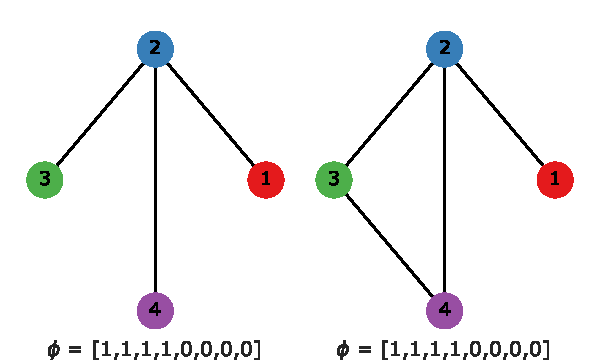
\includegraphics[width=0.32\textwidth]{assets/figures/wl_example/wl_iteration_0.pdf}\label{fig:wl_example_0}}
  \hfill
  \subfloat[After relabeling]{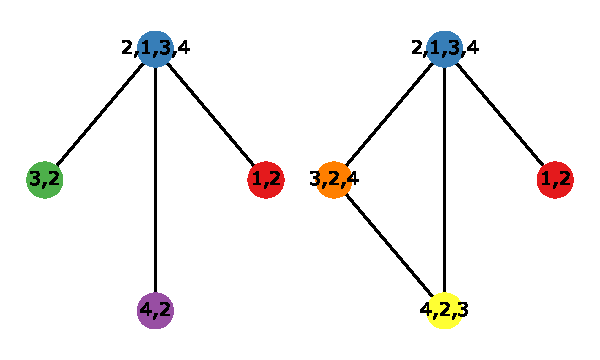
\includegraphics[width=0.32\textwidth]{assets/figures/wl_example/wl_iteration_1_stage_0_recolored}\label{fig:wl_example_1}}
  \hfill
  \subfloat[After label compression]{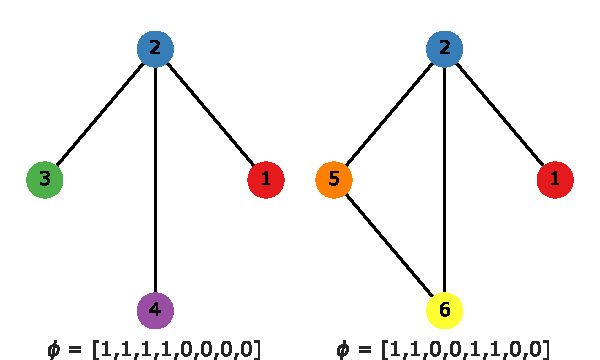
\includegraphics[width=0.32\textwidth]{assets/figures/wl_example/wl_iteration_1_stage_1_compressed.pdf}\label{fig:wl_example_2}}
  \caption{Weisfeiler Lehman algorithm example. This examples shows one WL iteration with two graphs. The initial graphs are shown in \textbf{(a)}. The first step of the iteration is relabeling the graph vertices by concatenating each node label with its sorted neighbourhood labels. The finished relabeled graph is shown in \textbf{(b)}. As an extension to the plain Weisfeiler-Lehman algorithm, we also show the label compression step where the long labels, consisting of the node label and its neighbourhood labels, get compressed into a smaller label by assigning each unique label a new number. Same labels in different graphs get the same new label. The result of this step is shown in \textbf{(c)}. Under \textbf{(a)} and \textbf{(c)} we also added the feature maps $\phi{}$ for the graphs. Each entry in the vector corresponds to a label. If a vector entry is 1, it means that the corresponding label is present in the given graph. The inner product on the vectors of the graphs is the value of the Weisfeiler-Lehman graph kernel for these two graphs.
  In this case, the similarity before the iteration would be $\langle \phi(G_1), \phi(G_2) \rangle = \langle [1, 1, 1, 1, 0, 0, 0, 0], [1, 1, 1, 1, 0, 0, 0, 0] \rangle = 4$. After the relabeling, the value of the inner product is $2$.
  Before doing the WL iteration, the inner product on the feature maps simply returns the number of common labels. After the first iteration, the neighbourhood of each node and therefor the structure of the graph is also reflected in the feature map - resulting in a lower similarity in out example.
  Please note that these feature vectors are specific to these two graphs and their labels. The dimension of the vector corresponds to the sum of the number of vertices in the two graphs.}\label{fig:wl_example}
\end{figure}

\subsubsection{Kernel Methods and Kernel trick}
We have seen that a kernel can be used to calculate a measure of similarity between two objects, eg. graphs.
Some kernels can be expressed as an inner product $k(X, X') = \langle \phi(X), \phi(X') \rangle$ on two (implicit) vector representations of the objects $X$ and $X'$.
In this case, the vector representations $\phi(X)$ can be used in conventional classification algorithms.
Yet, calculating these representations is not always possible or feasible since the dimension of such a representation is quite high.
There is another approach for classification (and regression), the aforementioned kernel methods.
Kernel methods operate directly with the kernel values and do not use the implicit feature representations $\phi(X)$.
Instead, kernel methods use the similarities $k(X, X')$ directly.

One popular example of a kernel method is the Support Vector Machine, or SVM.
The SVM is able to use both vector representations of elements in the dataset or the pairwise similarities, the gram matrix, between them.
At training time, the gram matrix $A$ of all objects in the training set, $d_{train} = \{X_1, X_2, \ldots, X_n\}$, is calculated.
This gram matrix $A$ and the corresponding classes then get fed into the SVM which fits its coefficients to them.
After training, to predict the label for a given instance $X_{test}$, the pairwise similarities of t$X_{test}$ and all training examples are calculated, resulting in a vector $v = (k(X_{test}, X_1), k(X_{test}, X_2), \ldots, k(X_{test}, X\_n))$.
This vector $v$ is then fed into the SVM which predicts the label for $X_{test}$.
Note that this kernel method approach does not use explicit feature maps of the instances, only their pairwise similarities.
This feature of not needing to calculate the explicit feature map $\phi$ is called kernel trick.
It enables linear models, such as the SVM, to solve non-linear separable problems.

In our work, we will use both the kernelized version of the SVM, ie. learning with a gram matrix, as well as the version using an explicit feature map $\phi$.


\labelsubsection{Graph Kernel Based Text Classification}{subsec:graph_kernel_based_text_classification}
In this section, we will introduce related work and briefly recap the history of the field.

\todo{How did the field evolve?}
\todo{Hint related tasks}
\todo{What is the most related work, how do they differ from our approach}
\todo{Relate the other work to the new approach and work out their differences/results}
\todo{Other approaches to graph classification}
\todo{Mention other graphs}

\paragraph{``Shortest-Path Graph Kernels for Document Similarity" \cite{Nikolentzos2017a}}
The most similar and recent work to our approach that we found was \cite{Nikolentzos2017a}. In this work, the authors first create co-occurrence graphs out of the text. Next, they create the gram matrix for the graphs with their own graph kernel and use a SVM to classify them.

Their graph kernel is a combination of two sub-kernels:
\begin{enumerate}
    \item{\textit{Simple label matching}: the number of matching node labels are compared between the two graphs}
    \item{\textit{Shortest path}: generate a shortest-path graph, then compare the edges}
\end{enumerate}
Note that the simple label matching sub-kernel does not take the structure into account, while the second sub-kernel actually uses both.
Both sub-kernels return a number which is added to produce the final value of the kernel.

The shortest path sub-kernel works as follows:
\begin{enumerate}
    \item{Generate shortest-path graphs for the two given graphs: The shortest path graph of a given graph has the same nodes.
    The edges are added by calculating the shortest paths between all pairs of nodes in the original graph. An edge is added between two nodes in the shortest path graph if the shortest path length between these nodes in the original graph is below a given parameter $d$. The edge also gets a weight assigned, which is $\frac{1}{d}$}
    \item{Count the number of same edges in the both graphs: when two edges are the same, add the product of their edge weights to the similarity}
\end{enumerate}

\todo{Mention that they did NOT perform experiments to differentiate the performance of the subkernels! My guess is that most of the performance comes from the simple-set matching subkernel.}
\todo{Note that the shortest-path sub-kernel does not actually add a lot of performance?}
\todo{Why is this approach different to ours? Co-occurrence vs. concept map}

\paragraph{``Text Categorization as a Graph Classification Problem" \cite{Rousseau2015a}}
In this paper, the authors generate co-occurrence graphs out of different text classification datasets.
To classify the graphs, they introduce their own graph kernel which is also an instance of the aforementioned kernels that count the number of occurrences of sub-structures.
In this case, the sub-structures this kernel counts are frequent subgraphs, ie. subgraphs that occur frequently in the graphs of the dataset.
To get a set of most-frequent subgraphs in the dataset, they develop their own approach, using depth-first search and a labelling function for graphs that enables finding frequent subgraphs efficiently.
After extracting the sub-graphs from the dataset this way, they only retain subgraphs which occur more often in the dataset than some defined parameter, the support value.
This significantly reduces the number of considered sub-graphs since most subgraphs occur quite infrequently.
This extension is indeed needed since the number of possible sub-graphs grows super-linear with the number of nodes/edges and can render the subsequent counting of the sub-graphs in the dataset infeasible.
Also, considering all possible subgraphs in all graphs in the dataset would not only require significant computational resources but would also result in sparse feature vectors since most sub-graphs occur infrequently.
This, in turn, would harden the classifier training problem.

As another measure to lower the runtime complexity of their algorithm, they also first extract the main core of each co-occurrence graph and only extract sub-graphs from them, not from the whole graphs.
A $k$-core is a subgraph $G_k$ of graph $G$ where all vertices have a degree greater or equal to $k$. The main core of a graph is the $k$-core with the highest possible $k$.
Thus the main core is the most connected subgraph of graph $G$, which includes only the most ``important" vertices and their edges to each other.

So, after extracting the main-core of each co-occurrence graph and determining the set of most-frequent sub-graphs in the dataset, they count the occurrences of the most-frequent sub-graphs for each graph in the dataset.
This results in feature maps $\phi_i$ which contain the counts of each most-frequent sub-graph per co-occurrence graph.
These feature vectors together with the labels are then used to train a SVM and are used to subsequently predict new instances by creating their feature maps and then predicting the label with this trained SVM.

The authors evaluated the classification performance of their approach on several datasets, namely the WebKB corpus, a subset of the reuters-21578 corpus (named R8), the ling-spam dataset and a corpus of Amazon reviews.
In our work, we also use these and other datasets. In later sections, we will introduce then more thoroughly.

In the paper, the authors argue that only retaining the main-core does not greatly damage the classification performance, yet it significantly reduces the compute time.
They also stress the importance of choosing an adequate support value for the sub-graph mining, mentioning the trade-off between performance and considered features. The process of choosing an adequate support value can be done unsupervised and gets treated similar to hyperparameter tuning of, for example, SVM hyperparameters.

This paper is quite similar to our approach since it also poses the text classification task as a graph classification task. Yet, they consider only one type of graph, the co-occurrence graph of the underlying texts.
Also, they do not evaluate the effect of combining text- and graph features.
That said, they provide interesting comparisons of text- and graph based approaches, pointing out the similarity of n-grams with the relationships which are captured in co-occurrence graphs.

\paragraph{``Concept Graph Preserving Semantic Relationship for Biomedical Text Categorization" \cite{Gulrandhe2015}}
Graphs: extracted keywords/concepts (POS tagger, only nouns), mapping of concepts to UMLS database, extraction of relationship between them.

Nodes are get 4 different weight components: tf, idf, connectivity, \#connected components.

Kernel: number of shared edges

No results


\paragraph{``Text classification using Semantic Information and Graph Kernels" \cite{???}}
In this paper, the text classification task is also converted into a graph classification task.
The authors create a graph of the underlying text by extracting so-called \underline{D}iscourse \underline{R}epresentation \underline{S}tructures, or DRS, which capture the semantic relationships in the sentences of the underlying text.
A DRS consists of two parts, namely a set discourse referents, or entities, and conditions on these entities.
The example given in the paper constructs the DRS for the sentence ``He throws the ball", which results in the DRS with the entities $\{\text{He}, \text{ball}, \text{throws}\}$ which get renamed to $\{x1, x2, x3\}$.
The conditions then define the meaning or relationship of the items. In the given example the DRS conditions are $\{\text{male}(x1), \text{ball}(x2), \text{throws}(x3), \text{event}(x3), \text{agent}(x3, x1), \text{patient}(x3, x2)\}$.

\todo{How to cite this example?}

To construct a graph from the extracted DRS', the entities become vertices and the conditions become edges between them.
A unary condition on a vertex, for instance $\text{male}(x1)$, becomes a loop for the node $x1$.
Conditions on two entities become directed edges, going from the entity of the first argument to the second condition argument, for example the condition $\text{agent}(x3, x1)$ creates a node from $x3$ to $x1$.
This results in a graph which captures the semantic relationship between the entities of the underlying graph.
Note that edge node labels, or entities, are not as important as the edges , or conditions, between them.
This is accounted for in the kernel the authors use in the next step.
Also note, that the process of creating a DRS graph for a given text is independent of other texts and can easily be parallized.

After constructing DRS graphs for all texts in the dataset, the authors use a variant of a random-walk kernel, customized to capture the importance of the edges instead of the nodes.
In the plain random-walk kernel, random walks are done on the two graphs, $G$ and $G'$ and the counts of equal random walks are counted, resulting in a measure of similarity between these two graphs. The higher the count of equal random walks, the higher the similarity.
The equality of two walks is determined by comparing the labels of the visited nodes.
In the case of DRS graphs, this would not yield a good kernel since the labels of the nodes are placeholders, ie. two vertices with the same label, for example $x1$, can correspond to totally different entities.
So, the standard definition of walk equality can not be used in the case of DRS graphs.
Instead, the authors introduce an approach which, for a given node $v_1$ of graph $G$, returns an ``equal" node $v_2$ in graph $G'$ that has similar edge \textbf{labels}.
This enables the random-walk graph kernel to ``merge" nodes with different node labels, that is placeholder like $x1$, on the two graphs, thus enabling random walks with meaningful node equality in the case of the DRS graphs.
After extracting the gram matrix of the DRS graphs with this extended random-walk graph kernel, the authors then use a SVM to evaluate their approach on the \textit{reuters-21578} dataset.
They use only a subset of 50 texts in the five most frequent classes of the dataset as their corpus. Then they create the DRS graphs for these texts and randomly select 25 of each class to create a gram matrix.
This gram matrix then gets used to train a one-versus-one SVM classifier. So, they do binary classification and present the results of the performance of the pairs of the 5 classes they considered.
The authors explain the reason for this small number of considered documents and classes by mentioning the runtime complexity of their approach, most notably the runtime complexity of the random-walk kernel.
They also acknowledge that they do not provide baseline results or comparisons between different approaches to text-classification or results with other graph kernels.

That said, this work is also similar to our approach in the sense that they also use graphs representations of texts to classify.

\todo{Maybe create similar kernel which does link prediction by defining edge equality through similar source/destination node labels?}

\paragraph{``Deep Graph Kernels" \cite{Yanardag2015}}
In this paper, the authors introduce an extension for existing kernels for which the explicit feature map $\phi$ can be calculated.
When calculating the kernel
\begin{equation*}
k(G, G') = \phi^T(G) \cdot \phi(G')
\end{equation*}
they add a weighting matrix $M$
\begin{equation*}
k(G, G') = \phi^T(G) \cdot M \cdot \phi(G')
\end{equation*}

The intuition here is that each vector entry of $\phi(G)$ corresponds to the count of some substructure of $G$ and that these substructures are not independent of each other, ie. they can be similar to each other.
Yet when calculating the plain kernel only exact matches of substructures in the two graphs are considered.
For instances, suppose substructure $g_1$ is similar to another substructure $g_2$ and substructure $g_1$ is only present in $G$ and not in $G'$, conversely substructure $g_2$ is only present in $G'$ and not in $G$.
Suppose some kernel $k$ would construct $\phi_k(G)$ by counting the occurrences of $g_1$ and $g_2$, so $\phi_k(G) = (n_{g_1}(G), n_{g_2}(G))$ where $n_{g_i}(G)$ counts the occurrence of substructure $g_i$ in $G$.
In the above example, $\phi_k(G_1) = (1, 0)$ and $\phi_k(G_2) = (0, 1)$. When calculating $k(G, G') = \phi_k^T(G) \cdot \phi_k(G') $ the similarity under the kernel would equal 0, therefore ignoring the similarity of substructure $g_1$ and $g_2$.
The proposed extension to the kernel aims to address this issue by using embeddings for the substructures to identify the similarity of substructures and then allowing ``partial" instead of only exact matches.
In the above example, the new $\phi_{new}(G)$ would not be $(1, 0)$ but $(1, i)$ and $\phi_{new}(G') = (i, 1)$ with some $i > 0$.
In our example, the aforementioned matrix $M$ would be
\begin{align*}
M = \begin{bmatrix}
1 & i \\
i & 1
\end{bmatrix}
\end{align*}

In this case, when calculating the kernel for these two graphs, the similarity would be $(1, 0)^T \cdot M \cdot (0, 1) = (1, 0)^T \cdot (i, 1) = i$ instead of $(0, 1)^T \cdot (1, 0) = 0$.
So, the augmented kernel between these graphs would actually capture the similarity of substructures instead of only using exact matches of them.

The authors then introduce two ways to create the matrix $M$ for a kernel, namely by creating it by hand using a measure of similarity between the substructures or by learning the embeddings with an approach similar to the \textit{word2vec} algorithm.
In both cases, the matrix $M$ aims to encode the similarities of the substructures.

The authors report an improvement of classification scores for several real-world datasets, comparing the scores of the plain version of a kernel with their augmented version.


\todo{How does this approach differ from ours?}